\chapter{Differential Geometry and Surface Curvature} \label{ch:diffgeo}


Our goal is establish a resource efficient method of finding curvilinear content in 2D grayscale digital images using concepts of differential geometry. We proceed by
\begin{enumerate*}[label=(\roman*)]
	\item establishing a standard method of viewing these images as 2D surfaces,
	\item developing a minimal yet rigorous distillation of differential geometry
			to obtain suitiable quantifiers
			for the study of curvilinear structure in 3D surfaces,
	\item establishing a filter based on these quantifiers,
	and finally
	\item developing methods necessary for efficient computation of the filter.
\end{enumerate*}


%%%%%%%%%%%%%%%%%%%%%%%%%%%%%%%%%%%%%%%%%%%%%%%%%%%%%%%
\section{Problem Setup in Image Processing}\label{sec:image-processing-setup}

%\vcomment{This section should be basically describing how to view an image as a surface.
%  Use any notation here that is useful beyond differential geometry, in all the contexts
%  we need to consider the image (in terms of Fourier Theory, scale space theory,
%  Frangi filtering, etc. all together.}
A digital 2D grayscale image is given by a $M\times N$ array of pixels, whose intensity is given by an integer value between 0 and 255. For simplicity, we will rescale this intensity to be a real number between 0 and 1.

\begin{defn}[Image as a pixel matrix] \label{def:image_as_pixel_matrix}
	\begin{equation*}
	\img \in \N^{M \times N}
	\quad\textrm{with}\quad
	0 \le \img_{ij} \le 1
	\end{equation*}
\end{defn}
	% iI hate this wording.
	For theoretical purposes, we wish to consider any such picture to ultimately be a sampling of a 2D continuous surface. We also require that this surface is sufficiently continuous as to admit the existence of second partial derivatives.
	
\begin{defn}[Image as an interpolated surface] \label{def:image_as_surface}
 \begin{equation*}
 h: \R^2 \to \R
 \quad \textrm{with}\quad
 h \in \mathcal{C}^2\left(\R^2\right),
 \quad\textrm{where}\quad
    h(i,j) = \mathtt{I}_{ij}
    \; \forall (i,j) \in
     \left\{0,...,M\right\} \times
     \left\{0,...,N\right\} \subset \N^2
    \end{equation*}
\end{defn}
% say the same thing with words
That is, the function $h$ is identical to the pixel matrix $\img$ at all integer inputs,
and simply a ``smooth enough'' interpolation of those points for all other values.


It is of course necessary to admit that $\mathtt{I}$ is not really a perfect representation of the underlying ``content'' within the picture. Not only is information lost when $\img$ is stored as an integer, there are also elements of noise and anomalies of lighting that would constitute noise to the original signal. There are multiple treatments of image processing that do address this discrepancy in a pragmatic way \cite{DIPGW}, especially when the goal is noise reduction.
However, we will be content to simply represent the pixels of $\img$ as the ultimate ``cause'' of the surface $h$ in \cref{def:image_as_surface}, and worry not about how faithfully that sampling corresponds to the real world.
% Word salad, also rude? ask chang about this
Moreover, though our samples in the image domain have been carefully prepared (as outlined in \cref{sec:NCS-data-set}), there are numerous shortcomings therein, and improvements to the veracity of our original signal could be made from many angles.
Though we shall draw upon the notion of the pixel matrix $\img$ as a sampling again to motivate our development of scale space theory in \cref{ch:scale-space-theory}, we ultimately use these techniques because we find them successful to our problem. A view of an inset of an image sample as a three dimensional graph, as shown in \cref{fig:inset_surf}, supports our decision to link our images of concern with this  three dimensional interpretation. We mention here, whereas \cref{fig:inset_surf} shows these \textit{dark} curvilinear structures, i.e. ``valleys'' within the surface containing local minima, other image domains may be more concerned with \textit{bright} curvilinear structures, i.e. ``ridges'' within the surface. Although our images of interest in this thesis are indeed dark curvilinear structures, we shall occassionally refer to surfaces where bright curvilinear structures are the concern, especially in \cref{sec:calculate-weinmap-of-a-ridge} and \cref{ch:unifrangi}. We do so only for ease of visualization. We will discuss the differences between these two structures in \cref{ch:unifrangi} and provide a way to distinguish between them.

\begin{figure}[t]
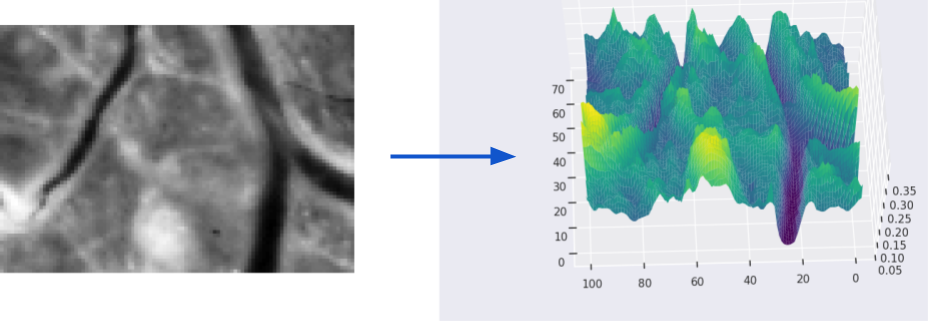
\includegraphics[width=\textwidth]{inset_surf}
\caption{Grayscale image (inset) as an interpolated surface}
\label{fig:inset_surf}
\end{figure}
 
%%%%%%%%%%%%%%%%%%%%%%%%%%%%%%%%%%%%%%%%%%%%%%%%%%%%%%%
%%%%%%%%%%%%%%%%%%%%%%%%%%%%%%%%%%%%%%%%%%%%%%%%%%%%%%%
\section{Differential Geometry} \label{sec:differential-geometry}
  
We wish to describe the structure of an image as a surface. To do this, we develop the notion of curvature of a surface in $\R^3$ in a standard way \cite{Kuhnel-DiffGeo}.

\subsection{Preliminaries of Differential Geometry}
%\vcleanup{Mention when you're talking about a general surface in $\R^3$ and when it's specifically a graph and make sure it's clear which case you're dealing with and motivate why you'd want to talk about things that aren't graphs at all (to define shape operator in general). Potentially rework to not talk about non-graphs when irrelevant. Although it's useful to keep some references to non-graphs to align this with "the general picture" and what you'll find in a diff geo textbook, also because I already wasted time doing the hard work.}
    Given an open subset $U\subset \R^2$ and a twice differentiable function  $h: U \to \R$ (as in \cref{def:image_as_surface})
    we define the graph, $f$, of $h$ in the following definition.
    
    \begin{defn} \label{def:graph}
    The surface $f$ is a graph (of the function $h$) when 
    \[
     f: U \to \R^3 \quad \textrm{by} \quad f(u_1, u_2) \;=\; \big(u_1 , u_2 , h(u_1,u_2)\big)
     \;,\quad u = (u_1, u_2) \in U \subset \R^2 \]
    \end{defn}
    %That is, $f$ is an embedding/immersion/parametrization of the function h
    Since the graph $f$ is clearly one-to-one (into $\R^3$) by definition, we may readily associate any input $u\in U$ with
    its corresponding output $p \in f[U]$, i.e.
    $ p = f(u) = f(u_1, u_2) \;=\; \big(u_1 , u_2 , h(u_1,u_2)\big)$,
    % world salad but may need motivation.
    depending on whether we wish to focus on a point of a graph in terms of its input
    or in terms of the structure of the graph itself.
    
    % Motivation
    Our development of curvature ultimately will hinge upon a careful consideration of the tangent plane of $f$ at a point $p$, for we will require a concrete definition of both the tangent space within the domain and image of $f$,
    as well as the differential" of $f$,
    % shit or not because we need it later!
    % the lattermost of which we will only define for the immediate case required.
	%    Seeing that $f$ is one-to-one should make a lot of this
	%    futzing about complete overkill, but I've yet to find a way to distill it.
	%    That is, this development works for any parametrized surface element, not necessarily a graph. Whatever for now.
    
    
    \begin{defn}[Tangent space of $U$ at $u$] \label{def:tangent-at-U}
    	\[ T_{u} U = \left\{u\right\} \times \R^2
    	\]
    	\end{defn}
    \begin{defn}[Tangent space of $\R^3$ at $p$] \label{def:tangent-of-R3}
    	\[ T_{p} \R^3 = \{p\} \times \R^3
    	\]
    \end{defn}
    It is immediately clear that $T_uU$ and $T_p\R^3$ are isomorphic to
    $\R^2$ and $\R^3$, respectively, and we can easily visualize elements of $T_uU$ are tangent vectors in $\R^2$ ``originating'' at the point $u$, and elements of $T_p\R^3$ are tangent vectors ``originating'' at the point $p$.
\begin{defn}[The differential of $f$ at a point $u$] \label{def:differential-map}
       	$Df\vert_u$ is the map from $T_uU$ into $\R^3$ given by
    \[
     Df|_u : T_uU \to T_{f(u)}\R^3
     \quad \textrm{by}
     \quad w \mapsto J_f (u) w
    \]
where $J_f(u)$ is the Jacobian of $f$ evaluated at some fixed point $u \in U$, i.e. the matrix
\[
J_f (u) = \left[ \left.\frac{\partial f_i}{\partial u_j}\right\vert_u \right]_{i,j}
\]
\end{defn} % You can in some ways argue that J_x(f) is a better notation
%Although not necessary presently, we could just as easily consider the differential of an arbitrary function as a map between tangent vectors in the function's domain and tangent vectors in its range.
We could also just identify the differential \cref{def:differential-map}  with a mapping $U \to \R^3$ by the obvious isomorphism inherent in \cref{def:tangent-at-U}. In this case, the differential of $f$ at $x$ is simply a linear transformation between the tangent spaces $T_uU$ and $T_p\R^3$ where the matrix of the transformation is given by the Jacobian. We can define such a differential at any point $u$ in the domain.

With these three definitions, we are equipped to give a formal definition of $T_uf$,
the tangent plane of $f$ at an input $u$.
\begin{defn}[Tangent plane of a graph]\label{def:tangent-plane}
\[
T_u f := Df\vert_u \left(T_u U\right)
\subset T_{f(u)} \R^3 = T_{p} \R^3
\]
\end{defn}

The vectors in this plane can thus be identified as tangent vectors from $T_uU$ that have been passed through the differential mapping $Df\vert_u$.
We shall denote a generic tangent vector $X \in T_u f$ at point $p$.
%%%%%STOPPEED HERE
We may expand any such vector $X$ in terms of the basis $\left\{ \frac{\partial f}{\partial u_i}\right\}_{i=1,2}$; that is,
$\textrm{span}\left\{ \frac{\partial f}{\partial u_1}, \frac{\partial f}{\partial u_2}\right\} = T_u f$. Each of these basis vectors are the columns of the Jacobian matrix and are \textit{parametric} derivatives of $f$ for the input $u$.  

% level of "needless" abstraction
Given the level of abstraction above, it may be refreshing to explicitly show the linear independence of this set in the case of an arbitrary graph $f$.
%it's the span though? just say it's the span?
\begin{lemma} \label{lemma:f_ui-is-a-basis}
	When $f$ is a graph, for all points $u \in U$, $\left\{\frac{\partial f}{\partial u_1} , \frac{\partial f}{\partial u_2}\right\}$ is in fact a basis for the tangent plane $T_uf$.
\end{lemma}

\begin{proof}
Given the definition of a graph $f$ as in \cref{def:graph}, we can directly calculate the parametric derivatives of $f$ at a point $u$.
\[
f_{u_1} = (1,0,h_{u_1}(u)) \quad\textrm{and}\quad f_{u_2} = (0,1,h_{u_2}(u))
\]
 which are obviously linearly independent.  Then $Df\vert_u (1,0) = f_{u_1} ,$ and $ Df\vert_u (0,1) = f_{u_2}$, which shows $\left\{\frac{\partial f}{\partial u_1} , \frac{\partial f}{\partial u_2}\right\} \in T_uf$.  Thus $\left\{\frac{\partial f}{\partial u_1} , \frac{\partial f}{\partial u_2}\right\}$ is a linearly independent subset of $T_u f$, and can serve as its basis.\end{proof}

Quite obviously, we're assuming $(1,0), (0,1) \in U$. If this is not the case, we pick some $\alpha$ small enough so that $(\alpha,0)$ and $(0,\alpha)$ are contained and this scaled version would serve as a basis instead.

	The parametric derivatives of $f$ are not, in general, orthogonal at any point $u$, unless it happens that $h_{u_1} $ or $h_{u_2}$ is zero.
	%A visualization of some of the above is given in \cref{fig:Tuf}, although note that $f_{u_1}$ and  $f_{u_2}$ accidentally appear orthogonal.
	
%	\begin{figure}\centering
%		\includegraphics[width=0.8\textwidth]{T_uf}
%		\caption{Tangent plane of a graph}
%		\label{fig:Tuf} 
%	\end{figure}
%  	But the above allows us to view $Df\vert_u$ differential map of $f$ is exactly the expansion of
%  	a point  $v \in U$ along the basis
%  	$\left\{\frac{\partial f}{\partial u_1} , \frac{\partial f}{\partial u_2}\right\}$ .

We now concern ourselves with developing the notion of curvature on a surface. First, we need to consider an arbitrary regular curve (i.e. differentiable, one-to-one, non-zero derivative) contained within the image of $f$. 
  	
  	% this isn't really a definition...?
 

\subsection{Curvature of a surface and its calculation}
In the context of a regular arc-length parametrized curve $c: I \to \R^3$ parametrized along some closed interval $I\in \R$
 (that is, a differentiable, one-to-one curve where $c'(s) = 1 \;\; \forall s \in I$), curvature at a point $s \in I$ is defined simply as the magnitude of the curve's acceleration: $\kappa(s) := \vnorm{c''(s)}$.
 
 To extend the notion of curvature of a surface $f$, we can consider the curvature of such an arbitrary curve embedded within the surface.
 
 \begin{defn}[Surface curve] \label{def:curve-on-a-surface}
 	Given a closed interval $I \subset \R$, we call the regular curve
 	$c: I \to \R^3$ a surface curve in the event that $\image(c) \subset \image(f)$ entirely. The one-to-one-ness of the graph $f$ ensures that we can define (for the given curve) an intermediary parametrization $\theta$  so that
 	$ c = f \circ \theta $. That is,
 	\[
 	\theta : I \to U \; \textrm{by} \; \theta(t) = \big(\theta_1(t), \theta_2(t)\big)
 	\]
 	so that $c(t) = f(\theta_c(t)) \;\forall t\in I,$
 	and $c[I] = f\left[\theta_c[I]\right]$.
 \end{defn}
 Note as well that the velocity of this particular curve lies within $T_u f$. This
 can be seen by an elementary application of chain rule:
 \begin{align}
 \frac{d c}{dt} &= \frac{d}{dt}\big[ f(\theta_c(t))\big] \nonumber \\
 &= \frac{d}{dt}\big[f(\theta_1(t), \theta_2(t))\big] \nonumber \\
 &= \theta_1'(t)\left( \frac{\partial f}{\partial u_1} \right) + 
 \theta_2'(t)\left( \frac{\partial f}{\partial u_2} \right) \in T_uf.
 \end{align}
 
 Considering the parameter $p \in I$ and its associated point $u = \theta_c(p)$, we wish to compare the curvatures of all (regular) surface curves passing through the point $u$ at some particular velocity.
 
 We now present a main result that provides a notion of curvature of a surface.

	\begin{theorem}[Theorem of Meusnier] \label{thm:meusnier}
		Given a point $u \in U $ and a tangent direction $X \in T_u f$,
  any regular curve on the surface $c: I \to \image(f)$ with $p\in I : \theta_c(p) = u$
  where $c'(p) = X$ will have the same curvature.
	\end{theorem}
	
	%\vtodo{provide a visualization of this}
	
	In other words, any two curves on the surface with a common velocity at a given point on the surface will have the same curvature. To prove this, we require one final definition.
	
	\begin{defn}[The Gauss Map] \label{def:gauss-map}
		The Gauss map at a point $u$  is the unit normal to the tangent plane
		\[\nu : U \to \R^3 \quad\textrm{by}\quad  \nu(u) :=
		\frac{\frac{\partial f}{\partial u_1} \times \frac{\partial f}{\partial u_2}}
		{\vnorm{\frac{\partial f}{\partial u_1} \times \frac{\partial f}{\partial u_2}}} \]
	\end{defn}
	Each partial above understood to be evaluated at the input $u \in U$; that is, we calculate $\left.\frac{\partial f}{\partial u_i}\right|_u$.
	The existence of the cross product in its definition makes it clear that $\nu \perp \frac{\partial f}{\partial u_i}$ each $i=1,2$. A simple dimensionality argument of $\R^3$ implies that these must exist in $T_uf$. However, we can also show it directly: 
%	\vcomment{at this point if you can prove $\left\{ \frac{\partial \nu}{\partial u_1}, \frac{\partial \nu}{\partial u_2}\right\}$ are linearly independent then do so, or just save for later, in which case don't use derivates at all}
	To show that $\left\{\frac{\partial \nu}{\partial u_1} , \frac{\partial \nu}{\partial u_2}\right\} \in T_u f$,
	first note that at any particular $u \in U$,
	$\inner{\nu}{\nu} = 1 \implies \frac{\partial}{\partial u_i} \inner{\nu}{\nu} = 0$,
	and so by chain rule $2\inner{\frac{\partial \nu}{\partial u_i}}{\nu} = 0
	\implies \frac{\partial \nu}{\partial u_i} \perp \nu $.
	Since $ \nu \perp \spn\left\{\frac{\partial f}{\partial u_i}\right\} $ as well (since $\nu$ its outer product), in  $\R^3$, this implies
	$\spn\left\{\frac{\partial \nu}{\partial u_i}\right\} = % not \parallel
	\spn\left\{\frac{\partial f}{\partial u_i}\right\}$.
	
	Thus, we have $\textrm{span}\left\{ \frac{\partial \nu}{\partial u_1}, \frac{\partial \nu}{\partial u_2}\right\} \subset T_u f$ as well and we can also use it as a basis.
  The Gauss map is intrinsic to the surface and irrespective of any particular curve through it.
	
	We are finally ready to prove \cref{thm:meusnier}, the Theorem of Meusnier.
	
	\begin{proof}
	Let $X\in T_u f$ be given and consider some curve where
  %$\frac{\partial c}{\partial t}(u) = X$ where $X \in T_u f$.
  $c'(p) = X$.
  We wish to decompose the curve's acceleration along the  orthogonal vectors $X$ and
	the Gauss map $\nu = \nu(u_1, u_2) =
		\frac{\frac{\partial f}{\partial u_1} \times \frac{\partial f}{\partial u_2}}
		{\vnorm{\frac{\partial f}{\partial u_1} \times \frac{\partial f}{\partial u_2}}}$ as in \cref{def:gauss-map}.
		Note that $X$ and $\nu$ are indeed orthogonal,
		as $ X \in \spn\left\{\frac{\partial f}{\partial u_i}\right\} = T_u f$, and
		$\nu \perp T_u f$).
	 We then have (at this fixed point $u=\theta(p)$)
		
		\begin{equation} \label{eq:meusnier_acceleration}
			c'' = \inner{c''}{X} X + \inner{c''}{\nu}\nu
			\end{equation}. 
	
	Because $c$ is a regular curve, we either have $c''=0$,
	or $c' \perp c''$, since $\vnorm{c'} = 1$ implies
	$0 = \frac{d}{dt} \inner{c'}{c'} = 2 \inner{c''}{c'} $. Thus
	
		\[ \inner{c''}{X} = \inner{c''}{c'} = 0 \]

	
	 and we can rewrite the second coefficient of \cref{eq:meusnier_acceleration} using the chain rule: % prove chain rule?
	\begin{gather}
  \begin{aligned}
		\inner{c''}{\nu} &=
		\frac{\partial}{\partial t}\left[ \inner{c'}{\nu} \right]
			- \inner{c'}{\frac{\partial \nu}{\partial t}} \\
			&= \frac{\partial}{\partial t}\left[ \inner{X}{\nu} \right]
			- \inner{c'}{\frac{\partial \nu}{\partial t}} \\
			&= 0 - \inner{X}{\frac{\partial \nu}{\partial t}}
			%&= \inner{X}{\wein X} = \mathbf{II}(X,X)
      \end{aligned}
			\end{gather}
	
	Thus, we can express the curvature at this point on our selected curve as
	\begin{align}
	%\vnorm{c''} = \mathbf{II}(X,X) \vnorm{\nu} = \mathbf{II}(X,X)
	\vnorm{c''} = \vnorm{\inner{c''}{X} X + \inner{c''}{\nu}\nu}
	&= \vnorm{0 + \inner{c''}{\nu}\nu}  \nonumber \\
	&= \abs{- \inner{X}{\frac{\partial \nu}{\partial t}}}\vnorm{\nu}  \nonumber \\
	&= \abs{- \inner{X}{\frac{\partial \nu}{\partial t}}}  \nonumber \\
	&=  \abs{\inner{X}{-\frac{\partial \nu}{\partial t}}} \label{eq:expand_accel_norm}
	\end{align}
	
  We may compute the quantity $-\frac{\partial \nu}{\partial t}$ that appears in
	\cref{eq:expand_accel_norm} via chain rule:
	\begin{align} \label{gaussmap_timederivative}
	-\frac{d \nu}{dt} &= -\frac{d}{dt}\big[\nu(u_1, u_2)\big] \nonumber \\
	&= -\frac{d}{dt}\big[\nu(\theta_1(t), \theta_2(t))\big] \nonumber \\
	&= \theta_1'(t)\left( - \frac{\partial \nu}{\partial u_1} \right) + 
	\theta_2'(t)\left( - \frac{\partial \nu}{\partial u_2} \right)
	\end{align}
	
	
	Since $\textrm{span}\left\{ - \frac{\partial \nu}{\partial u_i}\right\}_{i=1,2}$ as a subset of $T_u f$,  we can identify a linear transformation which maps the basis
	$\left\{ \frac{\partial f}{\partial u_i}\right\}_{i=1,2}$ to this basis.
  
  We call this map which the Weingarten map $\wein$.
	
	\begin{defn}[The Weingarten Map] \label{def:wein-map}
		\[
		\wein: T_u f \to T_u f 
		\quad \textrm{given by the composition} \quad
		\wein = D\nu \circ (Df)^{-1}.
		%\wein(\frac{\partial f}{\partial u_i})
		%	= - \frac{\partial \nu}{\partial u_i}
		%\quad i=1,2		
		\]
	\end{defn}
	That is, $\wein(\frac{\partial f}{\partial u_i}) = - \frac{\partial \nu}{\partial u_i} $ for $i=1,2$.
  %where the negative sign comes about from blind adherence to \cref{eq:gaussmap_dt_expanded} and \cref{eq:expand_accel_norm}.
  This allows us to rewrite the time derivative of the Gauss map \cref{gaussmap_timederivative} as
		\begin{align}
		-\frac{d \nu}{dt} &= 
		\theta_1'(t)\left( - \frac{\partial \nu}{\partial u_1} \right) + 
		\theta_2'(t)\left( - \frac{\partial \nu}{\partial u_2} \right) \nonumber\\
		&= \theta_1'(t)\left( \wein\left(\frac{\partial f}{\partial u_1}\right) \right) + 
		\theta_2'(t)\left( \wein\left(\frac{\partial f}{\partial u_2}\right) \right)\nonumber \\
		&= \wein\left[\theta_1'(t)\left( \frac{\partial f}{\partial u_1}\right)  + 
		\theta_2'(t)\left( \frac{\partial f}{\partial u_2} \right)\right] \nonumber\\
		&= \wein\left(\frac{d}{dt}\left[ f\left(\theta(t)\right)\right] \right)
		= \wein\left( \frac{d}{dt} \left[ c(t) \right] \right) = \wein\left(X\right)
		\end{align} 
		With this, we can re-express the curvature of our curve from
		\cref{eq:expand_accel_norm} as the much simplified
		
		\begin{equation} \label{eq:expand_accel_norm_final}
		\vnorm{c''} = \abs{\inner{X}{-\frac{\partial \nu}{\partial t}}}
                = \abs{\inner{X}{\wein(X)}}
		\end{equation}
		
	
	The linear transformation $\wein$ from \cref{def:wein-map}, and thereby
	the computation of curvature given in \cref{eq:expand_accel_norm_final},
	depends only on the point $u$ and the selected direction $X$, not on the particular curve $c$ at all.
	\end{proof}
	To recap, given a point $u$ on the surface and an arbitrary vector $X$ in the tangent plane, we can calculate the curvature of any surface curve with velocity $X$ there. In fact, we refer to this intrinsic quantity as the normal curvature of the surface.
	
	\begin{defn} \label{def:normal-curvature}
		The normal curvature of a surface, denoted $\kappa_\nu$ at point $u$ in the direction $X$ is given by
		\[\kappa_\nu :=  \inner{X}{\wein(X)} \]
	\end{defn}
	In fact, \cref{thm:meusnier} shows that the normal curvature is an intrinsic property of the surface--it depends only on the
	surface at a point, and no reference to any particular curve on the surface is necessary or implied.
%	In other contexts (not necessary here), this quantity is referred to as the \textit{second fundamental form} at the point $u \in U$; that is, $ \mathbf{II}(X,X) := \inner{X}{\wein(X)}$.
	
	
	The map $\wein$ introduced in the proof above is known as the Weingarten map
	and is implicitly defined at each $u \in U$. 
	We wish to make its existence rigorous as well as find a matrix representation for it, using the standard motivation that $\wein(\frac{\partial f}{\partial u_i}) = - \frac{\partial \nu}{\partial u_i}$.
	
	
	That is, we may trace any $X \in T_u f$ which has been expanded in terms of the basis 
	$\left\{\frac{\partial f}{\partial u_1} , \frac{\partial f}{\partial u_2}\right\}$
	and map it to the basis $\left\{-\frac{\partial \nu}{\partial u_1} , -\frac{\partial \nu}{\partial u_2}\right\}$. 
	
	The Weingarten map can be formally shown to be well-defined, invariant under coordinate transformation in the general case (that is, for surfaces $f$ that are not graphs). We refer to \cite{Kuhnel-DiffGeo} for the general proof. Our present situation is much less delicate, as we're only concerned for cases when $f$ is a graph. In this case, the linear transformation may be simply constructed, and we proceed by simply calculating its matrix representation.	
	\begin{lemma}
		The Weingarten map as in \cref{def:wein-map} is well-defined for graphs.
	\end{lemma}
	To find a matrix representation for $\wein$ (which we will denote $\weinmat \in \R^{2\times2}$), we simply wish to find a linear transformation
	such that
	$\weinmat \left.\frac{\partial f}{\partial u_i}\right|_{T_u f}
		= - \left.\frac{\partial \nu}{\partial u_i}\right|_{T_u f} \quad \textrm{for} \; i=1,2$
			where $- \left.X\right|_{T_u f}$ denotes that $X \in T_u f$ is being represented in 
	local coordinates for $T_u f$ (Strictly speaking, of course $T_u f \subset \R^3$ and thus
	$\frac{\partial f}{\partial u_i} \in \R^3.$ Thus when we say $ \left.\frac{\partial f}{\partial u_i}\right|_{T_u f}$ we are referring to this 3-vector expanded with respect to the two-dimensional basis for $T_u f$). In matrix form, we describe this situation as
	
	\begin{align}
	\Bigg[ \;\weinmat\; \Bigg]
	\left[ \mcol{\left.\frac{\partial f}{\partial u_1}\right|_{T_u f}} \;
			\mcol{\left.\frac{\partial f}{\partial u_2}\right|_{T_u f}} \right]
			&= \left[ \weinmat \mcol{\left.\frac{\partial f}{\partial u_1}\right|_{T_u f}} \;
			\weinmat \mcol{\left.\frac{\partial f}{\partial u_2}\right|_{T_u f}} \right] \\
			&= \left[ \mcol{ \left.-\frac{\partial \nu}{\partial u_1}\right|_{T_u f}} \;
			\mcol{\left.-\frac{\partial \nu}{\partial u_2}\right|_{T_u f}} \right]
			\end{align}
			Now, representing each vector in  $T_u f$ with respect to the basis $\left\{ \frac{\partial f}{\partial u_i}\right\}$, we have
  \begin{align}
      	\Bigg[ \;\weinmat\; \Bigg]
      \left[ \mcol{\left.\frac{\partial f}{\partial u_1}\right|_{T_u f}} \;
      \mcol{\left.\frac{\partial f}{\partial u_2}\right|_{T_u f}} \right]
      = 
			\Bigg[ \;\weinmat\; \Bigg]
			\begin{bmatrix} - \frac{\partial f}{\partial u_1} - \\
				- \frac{\partial f}{\partial u_2} -
							\end{bmatrix}
			\left[ \mcol{\frac{\partial f}{\partial u_1}} \;
				\mcol{\frac{\partial f}{\partial u_2}}\right]
				= \begin{bmatrix} - \frac{\partial f}{\partial u_1} - \\
				- \frac{\partial f}{\partial u_2} -
				\end{bmatrix}
				\left[ \mcol{-\frac{\partial \nu}{\partial u_1}} \;
				\mcol{-\frac{\partial \nu}{\partial u_2}}\right] \\
	\end{align}
		 
	We can simplify this greatly by defining 
	\begin{equation}\label{fundamentalformcoefficients}
	g_{ij} := \inner{\frac{\partial f}{\partial u_i}}{\frac{\partial f}{\partial u_j}}
	\quad \textrm{and}\quad
	h_{ij} := \inner{\frac{\partial f}{\partial u_i}}{-\frac{\partial \nu}{\partial u_j}}
	\end{equation}
	
	so that
	\begin{equation}
	\Bigg[ \;\weinmat\; \Bigg]
	\begin{bmatrix} g_{11} & g_{12} \\ g_{21} & g_{22} \end{bmatrix}
	= \begin{bmatrix} h_{11} & h_{12} \\ h_{21} & h_{22} \end{bmatrix}
	\end{equation}
	
	Then we rearrange to solve for $\weinmat$ as
		\begin{equation} \label{weinmatconstruction}
		\weinmat
		\;=\; \begin{bmatrix} h_{11} & h_{12} \\ h_{21} & h_{22} \end{bmatrix}
		\left.\begin{bmatrix} g_{11} & g_{12} \\ g_{21} & g_{22} \end{bmatrix}\right.^{-1}
		\end{equation}
	
	where $\left[ g_{ij} \right]$ is clearly invertible, as the set
	$\left\{\frac{\partial f}{\partial u_j}\right\}$ is linearly independent.
	
	It should be noted that this matrix representation is accurate not only for the surface of a graph, but for any \textit{generalized} surface
	$f: U \to \R^3 $ with $u \mapsto (x(u), y(u), z(u))$ as well. We shall later show that this calculation simplifies (somewhat) in the case that our surface is a graph.
	
	Our final goal is to characterize such normal curvatures.
	Namely, we wish to establish a method of determining in which directions an extremal normal curvature occurs.
	
	
	\subsection{Principal Curvatures and Principal Directions}
	To do so, we shall consider the relationship between the direction $X$ and the normal curvature $\kappa_\nu$ \cref{def:normal-curvature} in that direction at some specified $u$.


	
	First, we need the following lemma:
    \begin{lemma}
        If $A\in R^{n\times n}$ is a symmetric real matrix, $v \in R^n$
        and given the dot product $\inner{\cdot}{\cdot}$,
        we have $\nabla_{v} \inner{v}{Av} = 2Av$.
        In particular, when $A = I$ the identity matrix, we have
        $ \nabla_{v} \inner{v}{v} = 2v$.
    \end{lemma}
    
    \begin{proof}
        The result is uninterestingly obtained by tracking
        each component of
        $\nabla_{v} \inner{v}{Av}$:
        
        \begin{align}
        {\Big(\nabla_{v} \inner{v}{Av}\Big)}_{i} =
                \frac{\partial}{\partial v_i} \Big[
                \inner{v}{Av}\Big]
                &=  \frac{\partial}{\partial v_i} \left[
                    \sum_{j=1}^{n} v_j {(Av)}_j\right] \\
                &=	\frac{\partial}{\partial v_i} \left[
                \sum_{j=1}^{n} v_j \sum_{k=1}^n a_{jk} v_k \right] \\
                &= \frac{\partial}{\partial v_i} \left[
                a_{ii} v_i^2 + v_i \sum_{k\ne i} a_{ik} v_k
                 + v_i \sum_{j\ne i} a_{ji} v_j
                 + \sum_{j\ne i} \sum_{k \ne i} v_j a_{jk} v_k \right] \\
    &=  2 a_{ii} v_i + \sum_{k\ne i} a_{ik} v_k
    + \sum_{j\ne i} a_{ji} v_j + 0 \\
    &= 2 a_{ii} v_i + 2 \sum_{k\ne i} a_{ik} v_k
     = 2 \sum_{k=1}^n a_{ik}v_{k} = 2 {\big(Av\big)}_i \\
     &\quad \implies \nabla_{v} \inner{v}{Av} = 2Av.
        \end{align}
    \end{proof}
    
    We are now ready for the major result of this section, which ties the Weingarten map to the
    notion of normal curvatures.
    
    \begin{theorem}[Theorem of Olinde Rodrigues]
       	Fixing a point $u \in U$, a direction $X \in T_u f $ minimizes the normal curvature $\kappa_\nu = \inner{\wein X}{X}$ subject to $\inner{X}{X}= 1$
       	iff $X$ is a (normalized) eigenvector of the Weingarten map $\wein$.
       	\end{theorem}
    \begin{proof}
       	%	Recall first the definition of the first two fundamental forms,
       		%$\textbf{II}(X,X) = \inner{\wein{X}}{X}$
       	%	and $\textbf{I}(X,X) = \inner{X}{X}$.
       		In the following, we will assume that $X \in T_u f$ is expanded,
       		in local coordinates, i.e. along  a two dimensional basis
       		(such as $\left\{ \frac{\partial f}{\partial u_i}\right\}_{i=1,2}$
       		) and thus can refer to $\wein$ freely as the $2\times2$ matrix $\weinmat$.
       		Using the method of Lagrange multipliers, we define the Lagrangian:
       		\begin{equation}
       		\mathscr{L}(X; \lambda) :=
        	\inner{\weinmat X}{X} - \lambda\Big(\inner{X}{X} - 1\Big) 
     \end{equation}
        	
        	Extremal values occur when
        	$\nabla_{X,\lambda} \mathscr{L}(X;\lambda) = 0$,
        	which results in the two equations
        	
     \begin{equation} \label{lagrange_requirements}
     \left\{ \begin{aligned}
      \nabla_X \inner{\weinmat X}{X} - \lambda \nabla_X \left( \inner{X}{X} - 1 \right) = 0 \\
      \inner{X}{X} - 1 = 0
     \end{aligned} \right.
     \end{equation}
     
     The second requirement is simply the constraint that $X$ is normalized.
     Using the previous lemma, we can simplify the first result as follows:
     
     \begin{gather}
     \nabla_X \inner{\weinmat X}{X} - \lambda \nabla_X \left( \inner{X}{X} - 1 \right) = 0 
     \nonumber \\
     2\weinmat X - \lambda \left(2 X \right) = 0  \nonumber \\
     \implies \quad \weinmat X - \lambda X = 0 \nonumber \\
     \implies \quad \weinmat X = \lambda X
     \end{gather}
     which implies that $X$ is an eigenvector of  $\weinmat$ with corresponding eigenvalue $\lambda$ ($X\ne 0 $ from the second equation of \cref{lagrange_requirements}).
     Thus the two hypotheses are exactly equivalent when $X$ is normalized. It is also worth remarking that the corresponding eigenvalue $\lambda$ is the Lagrangian multiplier itself.
       	\end{proof}
       	
       	Thus, to find the directions of greatest and least curvature of a surface at a point $u \in U$, we simply must calculate the Weingarten map and its eigenvectors. We refer to these directions as follows.
       	
       	\begin{defn}[Principal Curvatures and Principal Directions]
       		The extremal values of normal curvature of a surface at a point  $u\in U$
       		are referred to as \textbf{principal curvatures}. The corresponding directions at which normal curvature attains an extremal value are referred to as \textbf{principal directions}.
       	\end{defn}
       	
       	Our final goal is to explicitly determine a (hopefully simplified) version of the Weingarten map in the case of a graph $f(u_1,u_2) = (u_1,u_2, h(u_1,u_2))$ and calculate
       	the principal directions and curvatures in a simple example.
       	        		
       	\begin{theorem}[Weingarten Map of a Graph]
        	Given the graph $f: U \to \R^3$ where $(x,y) \mapsto (x, y, h(x,y))$, the matrix
        	representation of its Weingarten map is given by
        	\begin{equation} \label{weinmatexactgraph}
        	\weinmat = \Hess(h) \tilde{G} \;,\quad \mathrm{where} \quad
	        	\tilde{G} := \frac{1}{\left({1+h_x^2 + h_y^2}\right)^{3/2}}
	        	\begin{bmatrix}
		        	1 + h_y^2 & -h_x h_y \\
		        	-h_x h_y & 1 + h_x^2 \\
	        	\end{bmatrix} 
        	\end{equation}
        	
        	In particular, given a point $u = (x,y) \in U \subset \R^2$ where $h_x \approx h_y \approx 0$, we
        	have $\tilde{G} \approx \mathrm{Id}$, and thus $\weinmat \approx \Hess(h)$.
        	
       	\end{theorem}
       	\begin{proof}
       		We begin from \cref{weinmatconstruction}.
       		First, consider each component from \cref{fundamentalformcoefficients}
       		and rewrite via chain rule:
      		 \[ h_{ij} = \inner{\frac{\partial f}{\partial u_i}}{-\frac{\partial \nu}{\partial u_j}}
       		= \inner{\frac{\partial^2 f}{\partial u_i \partial u_j}}{\nu} \]
       		
       		Now, given our particular surface $f$, we can calculate each of these components directly. We have:
       		\begin{equation}
       		\begin{gathered}
       		f_{x} = (1, 0, h_x) , \quad
       		f_{y} = (0, 1, h_y)  \\
       		f_{xx} = (0, 0, h_{xx}) , \quad
       		f_{xy} = (0, 0, h_{xy}) = f_{yx} , \quad
       		f_{yy} = (0, 0, h_{yy})
       		\end{gathered}
       		\end{equation}
       		
       		and we have the unit normal vector (Gauss map)
       		\begin{align}
       		\nu(u_1, u_2) &=
       		\frac{\frac{\partial f}{\partial x} \times \frac{\partial f}{\partial y}}
       		{\vnorm{\frac{\partial f}{\partial x} \times \frac{\partial f}{\partial y}}} \\
       		&= \frac{(1, 0, h_x) \times (0, 1, h_y)}{\vnorm{(1, 0, h_x) \times (0, 1, h_y)}} \\
       		&= \frac{\left( -h_x , -h_y , 1 \right)}{\sqrt{h_x^2 + h_y^2 + 1}}
	 \end{align}
	 We then calculate each $h_{ij}$ as
	 \begin{equation}
	 \begin{gathered}
	 h_{11} = \inner{\frac{\partial^2 f}{\partial x^2}}{\nu} = 
		 \frac{h_{xx}}{\sqrt{1+h_x^2 + h_y^2}} \\
	  h_{12} = \inner{\frac{\partial^2 f}{\partial x \partial y}}{\nu} = 
	  \frac{h_{xy}}{\sqrt{1+h_x^2 + h_y^2}} = h_{21} \\
	  h_{22} = \inner{\frac{\partial^2 f}{\partial y^2}}{\nu} = 
	  \frac{h_{yy}}{\sqrt{1+h_x^2 + h_y^2}} \\
	 \end{gathered}
	 \end{equation}
	 
	 and thus the first matrix in \cref{weinmatconstruction} is given by
	 
	 \begin{equation} \label{hij_exactgraph}
	 [h_{ij}] = \frac{1}{\sqrt{1+h_x^2 + h_y^2}} \,  \Hess (h)
	 \end{equation}
	 
	 To calcuate the second, we use
	 
	 
	 
	 \begin{equation}
	 \begin{gathered}
	 g_{ij} = \inner{\frac{\partial f}{\partial u_i}}{\frac{\partial f}{\partial u_j}} \\
	 g_{11} = \inner{f_x}{f_x} = 1 + h_x^2 \\
	 g_{12} = \inner{f_x}{f_y} = h_x h_y = g_{21} \\
	 g_{22} = \inner{f_y}{f_y} = 1 + h_y^2
	 \end{gathered}
	 \end{equation}
	 
	 and thus
		\begin{equation} \label{gij_exactgraph}		 
		[g_{ij}]^{-1} = \begin{bmatrix} 1 + h_x^2 & h_x h_y \\
					h_x h_y & 1 + h_y^2 \end{bmatrix}^{-1}
					\;=\;	\frac{1}{1+h_x^2 +h_y^2}
					\begin{bmatrix} 1 + h_y^2 & -h_x h_y \\
					-	h_x h_y & 1 + h_x^2 \end{bmatrix}
		\end{equation}
       	
       	Combining $[h_{ij}]$ and $[g_{ij}]^{-1}$ from \cref{gij_exactgraph} and \cref{hij_exactgraph}
       	we arrive at our result, \cref{weinmatexactgraph}.
       	\end{proof}
       	
  We stress that this map $\wein$ is defined for each point $u \in U$.
  In the particular case that $u \in  U$ is a critical point, where $\nabla h(u) = (h_x(u), h_y(u)) = 0$, then it is clear from the previous theorem that $\weinmat$ is exactly the Hessian matrix $\Hess(h)$. Of course this implies that $\weinmat$ and $\Hess{(h)}$ have the same eigenvalues and eigenvectors at any such point.

%FIX_THIS % % % % % % % % % % % % % % % % % % % % % % % %
%But this observation is more broadly useful than for analyzing critical points alone. If $\tilde{G}$ above is close to identity, then the eigenvalues and eigenvectors of $\weinmat$ will be similarly close to the eigenvalues of the Hessian. We can rewrite $\tilde{G}$ from \cref{weinmatexactgraph} as identity plus a small matrix:
%\begin{equation}
%\tilde{G} = \frac{1}{1+h_x^2 +h_y^2}\left(I + [\delta]\right), \quad
%	[\delta] 	:= \begin{bmatrix} h_y^2 & -h_x h_y \\
%					  -h_x h_y & h_x^2 \end{bmatrix}
%\end{equation}
%
%We can then rewrite \cref{weinmatexactgraph} as 
%\begin{equation}
%\weinmat = \frac{1}{\left(1+h_x^2 + h_y^2\right)^{3/2}}\left( \Hess(h)
%+  \Hess(h) [\delta]\right)
%\end{equation}
%
%We can see that as $h_x, h_y$ are close to zero, $[\delta]$ will be very close to the zero matrix, and the constant $\left(1+h_x^2 + h_y^2\right)^{-3/2}$ will be very close to 1 as well, so we should not expect the addition of a "close to 0" matrix to have much effect on the eigenvectors or eigenvalues. This intuition is confirmed by a result from Wilkinson \cite{wilkinson-eigenvalue}, which we state without rigorous proof.
%
%% see wilkinson pg 66
%\begin{theorem}
%	If $A$, $B$ are matrices such that $\abs{A_{ij}} < 1 , \abs{B_{ij}} < 1$ (a condition that can be ignored with scaling) and $\lambda$ is a simple eigenvalue of $A$, then given $\epsilon > 0$, there exists a simple eigenvalue $\tilde{\lambda}$ of the matrix $A + \epsilon B$ with $\abs{\lambda - \tilde{\lambda}} = \bigO(\epsilon)$. Similarly, if $v$ is an eigenvector of A, then $\tilde{v}$ is an eigenvector of $A + \epsilon B$ with
%	$\abs{v - \tilde{v}} = \bigO(\epsilon)$.
%\end{theorem}
%
%The proof ultimately relies on a general result of analysis, that the zeros of a polynomial are continuous with respect to its coefficients. In this case, the polynomial in question is the characteristic polynomial
%$p(\lambda) = \det(\lambda I - A - \epsilon B)$, whose coefficients will scale with $\epsilon$. Thus $\weinmat \approx \Hess(h)$ for any point where the gradient $\nabla h \approx 0$. We shall see that we're only concerned with regions where $h_x, h_y$ is small anyway, and we do not expect much response anyway when the gradient is large. 
%
%We can bound the perturbation of eigenvalues from $\weinmat$ to $\Hess(h)$ by another result
%which we state without proof \cite{matrix-analysis-horn}.
%
%\begin{theorem}
%	Let A be a $n\times n$ normal matrix with eigenvalues $\lambda_1, \dots, \lambda_n$ and $E$ an $n \times n$ arbitrary matrix. If $\hat{\lambda} $ in an eigenvalue of $A + E$, then there is an eigenvalue $\lambda_i$ of A for which
%		$\abs{\hat{\lambda} - \lambda_i} \leq \vnorm{E}_2$
%\end{theorem}
%
%In the event that we do wish to rigorously compute the Weingarten map--that is, without concern for the magnitude of the gradient--we refer to \cite{jiao2008consistent} and survey papers mentioned therein.

  
  To make the Weingarten map and its relationship to the Hessian more explicit, we will calculate the Weingarten map for a relatively simple graph.
  
  \subsection{The Weingarten map and Principal Curvatures of a Cylindrical Ridge} \label{sec:calculate-weinmap-of-a-ridge}
  
  Let $f$ be the graph given by 
  \begin{equation}
   f: \R^2 \to \R^3 \;\textrm{by}\; f(x,y) = (x,y,h(x,y)), \;\textrm{with}\;
   h(x,y) = \begin{cases}
    \sqrt{r^2 - x^2} & -r < x < r \\
    0 & \textrm{else}
    \end{cases}
  \end{equation} 
  \begin{figure}[h!]
  \includegraphics[width=\linewidth]{circular_trough_with_axes_vectors}
  \caption{The graph of a cylindrical ridge of radius $r$}
  \label{fig:ridge-graph}
  \end{figure}
  
  
  The graph $f$ is depicted in \cref{fig:ridge-graph}. We calculate the necessary partial derivatives of $h(x,y)$ and apply them to \cref{weinmatexactgraph}.
  
%  \begin{gather}
%  \frac{\partial f}{\partial x} = \left(1, 0, \frac{-x}{\sqrt{r^2 - x^2}}\right)
%  \quad , \quad
%  \frac{\partial^2 f}{\partial x^2} = \left(0, 0, \frac{-r^2}{\left(\sqrt{r^2 - x^2}\right)^3}\right) \\
%  \frac{\partial f}{\partial y} = \left(0, 1, 0\right)
%  \quad , \quad
%  \frac{\partial^2 f}{\partial y^2} = \frac{\partial^2 f}{\partial x \partial y} = 0
%  \end{gather}
%  The gauss map is given by
%  \begin{gather}
%  \nu(x,y) = \frac{\frac{\partial f}{\partial x} \times \frac{\partial f}{\partial y}}
%  {\vnorm{\frac{\partial f}{\partial x} \times \frac{\partial f}{\partial y}}}
%  = \left( \frac{x}{r} ,\; 0 ,\; \frac{\sqrt{r^2 - x^2}}{r} \right) \\
%\implies
%\frac{\partial \nu}{\partial x}
% = \left(\frac{1}{r} \;,\; 0\;,\; \frac{-x}{r\sqrt{r^2-x^2}}\right)
% \quad , \quad \frac{\partial \nu}{\partial y} = \left(0,0,0\right).
%  \end{gather}
%  
%  We then calculate matrix elements of the Weingarten map's construction as given in
%  \cref{hij_exactgraph} and \cref{gij_exactgraph} :
%  \begin{align}
%  [h_{ij}] = \frac{1}{\sqrt{1+h_x^2 + h_y^2}} \,  \Hess (h)
%     &= \frac{1}{\sqrt{1+\left(\frac{x^2}{r^2-x^2}\right)}}
%     \begin{bmatrix}
%     \frac{-r^2}{\sqrt{r^2 - x^2}^3} & 0 \\
%    0 & 0
%     \end{bmatrix} 
%     = \begin{bmatrix}
%     \frac{-r}{r^2 - x^2} & 0 \\
%     0 & 0
%     \end{bmatrix} \
%     [g_{ij}]^{-1} &= \begin{bmatrix} \frac{r^2 - x^2}{r^2} & 0 \ 0 & 1 \end{bmatrix} \\
%     \implies \weinmat = [h_{ij}]	[g_{ij}]^{-1} &=
%     \begin{bmatrix}
%     \frac{-r}{r^2 - x^2} & 0 \\
%     0 & 0
%     \end{bmatrix} \begin{bmatrix} \frac{r^2 - x^2}{r^2} & 0 \ 0 & 1 \end{bmatrix} \\
%     &= \begin{bmatrix} - \frac{1}{r} & 0 \\ 0 & 0 	\end{bmatrix}	       	
%  \end{align}
\begin{gather*}
h_x = \frac{-x}{\sqrt{r^2 - x^2}}
\quad , \quad
h_{xx} = \frac{-r^2}{\left(r^2 - x^2\right)^{3/2}}\\
h_y = 0
\; , \quad
h_{yy} = 0 \;,\quad h_{xy} = 0
\end{gather*}

    \begin{align*}
  \weinmat &= \Hess(h)\tilde{G}
  = \frac{1}{\left(1+\frac{x^2}{r^2-x^2}\right)^{3/2}}
  \begin{bmatrix} \frac{r^2}{\left(r^2 - x^2\right)^{3/2}} & 0 \\
  0 & 0 \end{bmatrix} \\
  &= \frac{1}{\left(\frac{r^2}{r^2-x^2}\right)^{3/2}}
  \begin{bmatrix} \frac{r^2}{\left(r^2 - x^2\right)^{3/2}} & 0 \\
  0 & 0 \end{bmatrix}
%  = \frac{\left(r^2-x^2\right)^{3/2}}{r^3}
%  \begin{bmatrix} \frac{-r^2}{\left(r^2-x^2\right)^{3/2}} & 0 \\ 0 & 0 \end{bmatrix}
  = \cdots
  = \begin{bmatrix} \frac{-1}{r} & 0 \\ 0 & 0 \end{bmatrix}
  \end{align*}
  
The matrix of the Weingarten map and its eigenvalues (in local coordinates) and vectors are then
\begin{equation} \label{eq:trough-example-eigens}
  \weinmat = \begin{bmatrix} - \frac{1}{r} & 0 \\ 0 & 0 	\end{bmatrix} \quad
  u_2 = (1,0) \;,\; u_1 = (0,1) \quad
  \lambda_2 = \frac{-1}{r} \;,\; \lambda_1 = 0
  \end{equation}

The Theorem of Olinde Rodriguez then suggests that $u_2$ points in the direction of maximum curvature of the surface, $-\frac{1}{r}$, which is predictably in the direction directly perpendicular to the trough, whereas the direction of least curvature is along the trough and the curvature there is $0$. The Theorem of Meusnier, \cref{thm:meusnier}, suggests that the normal curvature $\kappa_2 = -\frac{1}{r}$ is reasonable--any curve on the trough perpendicular to the ridge should have the curvature of a circle, and the negative simply indicates that we are on the ``outside'' of the surface. Finally, we note that at the ridge of the trough is exactly where $\nabla f = 0$, and the Weingarten map is exactly the Hessian matrix there.

For arbitrary points $-r < x < r$, the Hessian takes the general form

\begin{equation}
\Hess(h) =
  \begin{bmatrix} \frac{-r^2}{\left(r^2 - x^2\right)^{3/2}} & 0 \\
                  0 & 0 \end{bmatrix}
\end{equation}

Its two eigenvectors are the same as in \cref{eq:trough-example-eigens},and its eigenvalues are $\lambda_2 = \frac{-r^2}{\left(r^2 - x^2\right)^{3/2}}$ and $\lambda_1 = 0$ and \cref{fig:ridge-graph}. Note that the leading eigenvalue is now a function of $x$.
% unfortunately, it's actually taking a maximal value as x is farther away from $x=0$ which is kind of unintuitive but i won't mention it here

%  \section{Orthogonality of Principal Directions and Approximated Principal Directions}
%    
%  \vcleanup{the eigenvectors of the Weingarten map are orthonormal. the eigenvectors of the hessian are also orthonormalizable. make the distinction!}
%  Our final point is to consider the relationship between the principal directions of a surface at a point. Viewing the surface in $\R^3$, we define the Hessian $\Hess(x,y)$ of the surface $L$
%  at a point $(x,y)$ on the surface as the matrix of its second partial derivatives:
%  \begin{equation}
%  \Hess(x,y) = \begin{bmatrix}
%  L_{xx}(x,y) & L_{xy}(x,y) \\
%  L_{yx}(x,y) & L_{yy}(x,y)
%  \end{bmatrix}
%  \end{equation}
%  
%  At any point $(x,y)$ we denote the two eigenpairs of the Hessian matrix of $h$ as
%  \begin{equation}
%  \Hess(x,y) u_i = \kappa_i u_i \; , \quad i = 1,2
%  \end{equation}
%
%  where $\kappa_i$ and $u_i$ are known as the
%  \textit{approximated principal curvatures} and \textit{approximated principal directions} of $L(x,y)$, respectively, and we label such that $|\kappa_2| \ge |\kappa_1|$. Notably, $\Hess(x,y)$ is a real, symmetric matrix (since  $L_{xy} = L_{yx}$ and $L$ is a real function) and thus its eigenvalues are real and its eigenvectors are orthonormal to each other, as given by following basic result from linear algebra
%  \cite{burden-faires}.
%  
%  % from burden and faires corollary 9.17
%  \begin{lemma}
%     	Let $A$ be a real, symmetric matrix. The eigenvalues of $A$ are real and its eigenvectors are orthonormal to each other.
%  \end{lemma}
%  
%  \begin{proof}
%     	Let $x\ne 0$ so that $Ax = \lambda x$. Then 
%     	\begin{align*}
%     	\vnorm{Ax}_2^2 = \inner{Ax}{Ax}  &= (Ax)^{*} Ax \\
%     	&= x^{*}A^{*}Ax = x^{*}A^T A x = x*A A x \\
%     	&= x^{*} A \lambda x = \lambda x^{*} A x \\
%     	&= \lambda x^{*} \lambda x = \lambda^2 x^{*} x = \lambda ^2 \vnorm{x}_2^2
%     	\end{align*}
%     	Upon rearrangement, we have
%     	$\lambda^2 = \frac{\vnorm{Ax}_2^2}{\vnorm{x}_2^2} \ge 0 \implies \lambda $ is real.
%     	
%     	To prove that a set of orthonormalizable eigenvectors exists,
%     	let $A$ be real, symmetric as above and consider the eigenpairs
%     	$Av_1 = \lambda_1 v_1$, $Av_2 = \lambda_2 v_2$ with $v_1, v_2 \ne 0$.
%
%     	5
%     	In the case that $\lambda_1 \ne \lambda_2$, we have
%     	\begin{align*}
%     	(\lambda_1 - \lambda_2)v_1^T v_2 &= \lambda_1 v_1^T v_2 - \lambda_2 v_1^T v_2 \\
%     	&= (\lambda_1 v_1)^T v_2 - v_1^T (\lambda_2 v_2) \\
%     	&= (Av_1)^T v_2 - v_1^T (Av_2) \\
%     	&= v_1^T A^T v_2 - v_1^T A v_2 \\
%     	&= v_1^T A v_2 - v_1^T A v_2 = 0
%     	\end{align*}
%     	Since $\lambda_1 \ne \lambda_2$, we conclude that $v_1^T v_2 = 0$.
%     	
%     	In the case that $\lambda_1 = \lambda_2 =: \lambda$, we can define
%     	(as in Gram-Schmidt orthogonalization) $u = v_2 - \frac{v_1^Tv_2}{v_1^Tv_1}v_1$.
%     	This is an eigenvector for $\lambda=\lambda_2$, as
%     	\begin{align*}
%     	Au &= A\left(v_2 - \frac{v_1^Tv_2}{v_1^Tv_1} v_1\right) \\
%     	&= A v_2 - \frac{v_1^Tv_2}{v_1^Tv_1} A v_1 \\
%     	&= \lambda v_2- \frac{v_1^Tv_2}{v_1^Tv_1} \lambda v_1 \\
%     	&= \lambda \left( v_2 - \frac{v_1^Tv_2}{v_1^Tv_1} v_1 \right) = \lambda u
%     	\end{align*}
%     	and is perpendicular to $v_1$, since
%     	\begin{align*}
%     	v_1^T u &= v_1^T\left(v_2 - \frac{v_1^Tv_2}{v_1^Tv_1}v_1\right) \\
%     	&= v_1^T v_2 - \left(\frac{v_1^Tv_2}{v_1^Tv_1}\right) v_1^T v_1 \\
%     	&= v_1^T v_2 - v_1^Tv_2 (1) = 0.
%     	\end{align*}
%  \end{proof}
%  
%  Thus we see that the two principal directions form an orthonormal frame at each point (x,y) within the continuous image $L(x,y)$.
  






    
   
    
   
 
 
